\documentclass[12pt]{article}

\usepackage{pablo}
\usepackage{multicol}

\usepackage[a4paper,margin=0.9cm]{geometry}

\usepackage{pablo-listings}

\usetikzlibrary{decorations.fractals}

\pagestyle{empty}

\begin{document}

\begin{center}
  Algorithmique

  {\large
    \textsc{Tortue}
  }

  ------------------
\end{center}

\section{Découverte d'IDLE}

\begin{multicols}{2}
\begin{enumerate}
  \item Ouvrir IDLE.
  \item Ouvrir un nouveau fichier : \texttt{File > New Window}.
  \item Dans la nouvelle fenêtre, recopier le programme de la colonne suivante.
\item Exécuter ce programme : \texttt{Run > Run module}.
\item Décrire ce que fait le programme.
\end{enumerate}

\columnbreak

\begin{lstlisting}[language=python,frame=single]
from turtle import *

forward(200)
left(90)
forward(100)
left(90)
forward(200)
left(90)
forward(100)

mainloop()
\end{lstlisting}

\end{multicols}

\section{Carré}

\begin{enumerate}
  \item Faire un programme qui dessine un carré
  \item Faire un programme qui dessine un pentagone régulier.
\end{enumerate}

\section{Boucles}

\begin{multicols}{2}
Le programme du dernier dessin était répétitif : on a recopié cinq fois la même chose. Plutôt que faire cela, on va dire à l'ordinateur de répéter cinq fois la même chose.

\begin{enumerate}
  \item Recopier et exécuter le programme de droite.
  \item En utilisant la même méthode, dessiner un polygone régulier à 10 côtés.
\end{enumerate}

\columnbreak

\begin{lstlisting}[language=python,frame=single]
from turtle import *

for i in range(4):
    forward(100)
    left(90)

mainloop()
\end{lstlisting}
\end{multicols}

\begin{enumerate}
  \setcounter{enumi}{2}
  \item Reproduire les dessins suivants.
\end{enumerate}

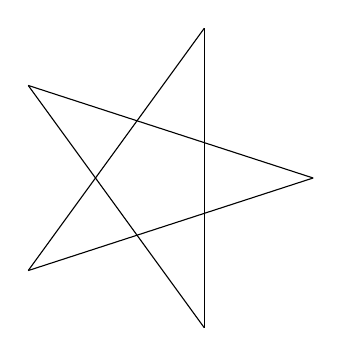
\begin{tikzpicture}[scale=2]
  \foreach \i in {1,...,5} {
    \draw ({\i *360/5}:1) -- ({(\i +2)*360/5}:1);
  }
\end{tikzpicture}
\hspace{\stretch{1}}
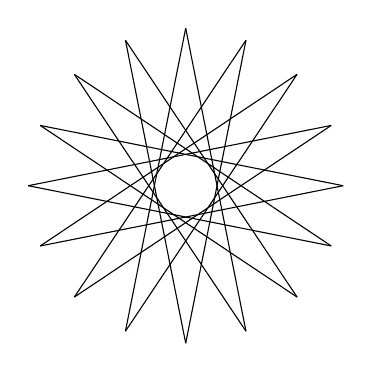
\begin{tikzpicture}[scale=2]
  \foreach \i in {1,...,16} {
    \draw ({\i *360/16}:1) -- ({(\i +7)*360/16}:1);
  }
\end{tikzpicture}
\hspace{\stretch{1}}
\begin{tikzpicture}[scale=1.5]
  \foreach \i in {1,...,6} {
    \begin{scope}[shift={(-1.5,5.5)},rotate={\i*360/6}]
      \draw (-0.5,-0.86602) -- (1.5,-0.86602) -- (1.5, -1.86602) -- (0.5,-1.86602) -- (0.5,-0.86602);
    \end{scope}
  }
\end{tikzpicture}

\section{Affectation}

~

\begin{multicols}{2}
On veut maintenant reproduire le dessin suivant.

\begin{center}
  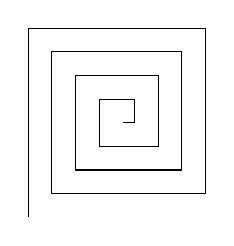
\begin{tikzpicture}[scale=0.15]
    \draw (0,0) -- ++(1,0) -- ++(0,2) -- ++(-3,0) -- ++(0,-4)
    -- ++(5,0) -- ++(0,6) -- ++(-7,0) -- ++(0,-8)
    -- ++(9,0) -- ++(0,10) -- ++(-11,0) -- ++(0,-12)
    -- ++(13,0) -- ++(0,14) -- ++(-15,0) -- ++(0,-16);
  \end{tikzpicture}
\end{center}

Pour cela, on va utiliser une variable \texttt{longueur}, qui représente la taille des segments, que l'on va augmenter peu à peu. Un code possible est donné à droite.

\columnbreak

\begin{lstlisting}[language=python,frame=single]
from turtle import *

longueur = 0

while longueur < 200:
    forward(longueur)
    left(90)
    longueur = longueur + 10

mainloop()
\end{lstlisting}

\end{multicols}

Reproduire le dessin suivant.
\begin{center}
  \begin{tikzpicture}[scale=0.5]
  \foreach \i in {1,...,5} {
    \draw ({(0.5*\i*\i)-0.5*\i},0) -- ++ (\i, 0) -- ++ (0,\i) -- ++(-\i, 0) -- cycle;
  }
  \end{tikzpicture}
\end{center}

\section{Marche de l'ivrogne}

\begin{multicols}{2}

  ~

  \begin{enumerate}
    \item Reproduire et exécuter le programme de droite.
    \item Que fait la fonction \texttt{randint} ?
    \item On s'intéresse au problème suivant : une tortue ivrogne essaye de traverser un pont sans garde-fou. À chaque pas, elle fait, au hasard, un pas en avant, un pas sur la droite, ou un pas sur la gauche. Malheureusement, le pont ne fait que trois pas de large. Modifier le programme pour qu'il s'arrête dés que la tortue ivrogne tombe du pont.
  \end{enumerate}

  ~

  \columnbreak

\begin{lstlisting}[language=python,frame=single]
from turtle import *
from random import randint

while True:
    alea = randint(-1,1)
    if alea == 0:
        forward(10)
    elif alea == -1:
        left(90)
        forward(10)
        right(90)
    else:
        right(90)
        forward(10)
        left(90)


mainloop()
\end{lstlisting}
\end{multicols}

\section{Pour aller plus loin (et au delà)}

\begin{multicols}{2}
  \noindent Reproduire le \emph{flocon de Von Koch} (figure de droite).

  \noindent Vous aurez besoin de fonctions (vous pouvez vous en passer, mais c'est plus compliqué). Vous avez droit à internet.

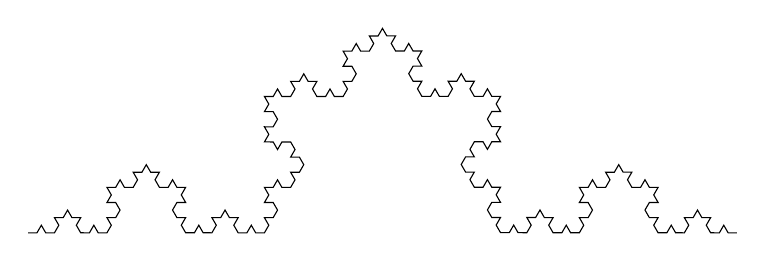
\begin{tikzpicture}[decoration=Koch snowflake,scale=3]
  \draw decorate{ decorate{ decorate{ decorate{ (0,0) -- (3,0) }}}};
\end{tikzpicture}
\end{multicols}

\end{document}
